\subsection{Influence of parameter choices on the resulting fingerprint}
\label{section:influenceOfParameters}
The influence of the main parameters could be the topic of a thesis on its own, so this subject is only discussed briefly.
\begin{figure}[H]
    \centering
    \begin{adjustwidth}{-2cm}{-2cm}  % je 2cm links und rechts in den Rand hinein
        \centering
        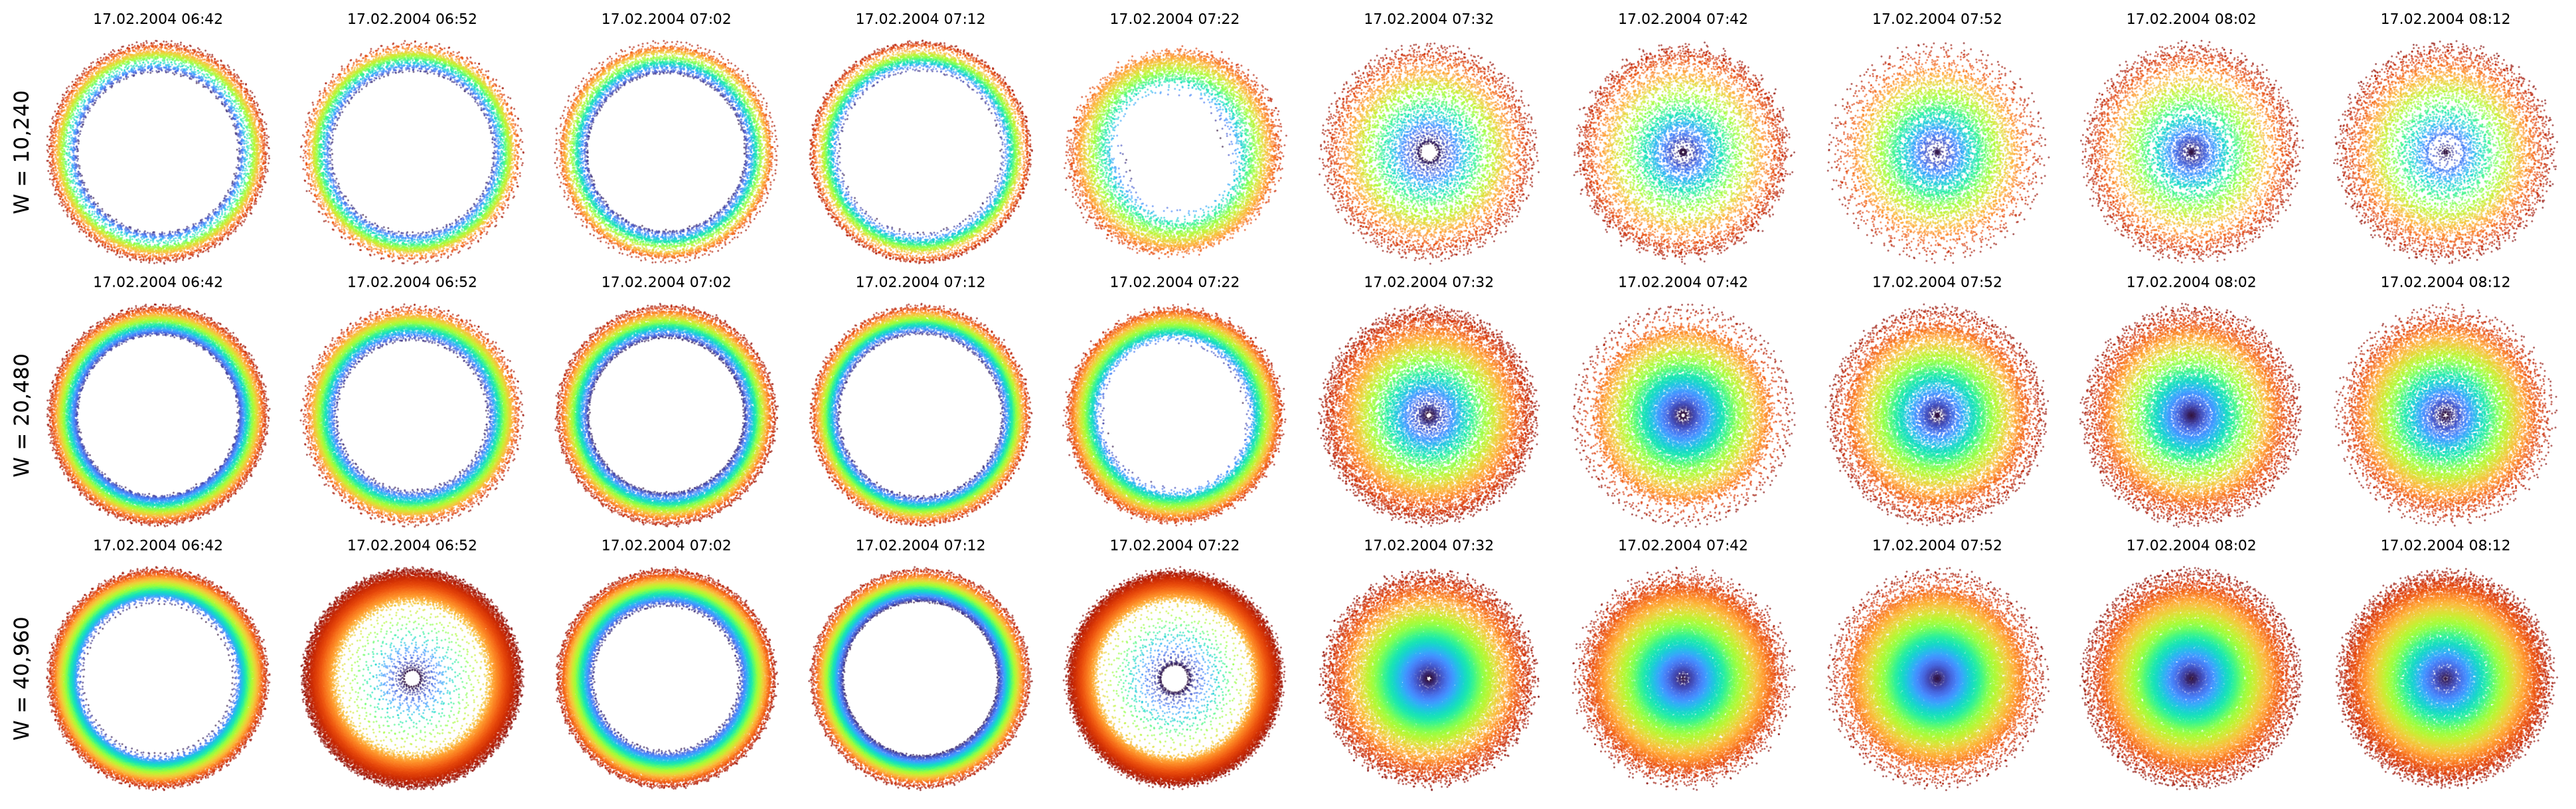
\includegraphics[width=\linewidth]{figures/differentParametersResults/window_compare_window_size.png}
    \end{adjustwidth}
    \caption{Influence of the parameter w on the plots.}
    \label{fig:differentW}
\end{figure}
As shown in \ref{fig:differentW} the window size has no significant influence on the overall shape of the fingerprint, but on the density of the point cloud. This was expected since the window size determines on how many samples are included in the calculation recalling the how many embedding vectors are used by $W - (d-1)\tau$ and each vector becomes one point of the fingerprint. For all tree representations the ring breaks at the same point in time. Choosing large windows does not visually improve anomaly detection as long as the window enough revolutions to determine its periodic behavior. At the same time larger windows keep older samples longer and therefore could react later to a significant change in the signal.  
Also the optimal representation in an visual anomaly tool is also a challenge on its own. The questions there which arise are: how many plots to use to give an optimal understanding on until now this form was dominant any deviations to this form could indicate a fault. A proposal for this issue would be to capture the healthy initial state of the machine after some time lock it and only plot further incoming data substitute this plots with new incoming data. As shown in \ref{fig:differentW} the window size has not a really significant influence on the shape of the fingerprint but more about how dense the cloud is. When recalling the knowledge that this parameter just influences how many data points get included into the calculation this makes sense because more points are included in the calculation thus more points have to be in the output. Choosing a really large window does not improve the anomaly detection because the data and thus its periodic behavior are captured on the same data. For $W = 40{,}960$ the window spans over exact two measurement files and therefore contains a jump in the signal that does not exist in a continuous measurement.
\begin{figure}[H]
    \centering
    \begin{adjustwidth}{-2cm}{-2cm}  % je 2cm links und rechts in den Rand hinein
        \centering
        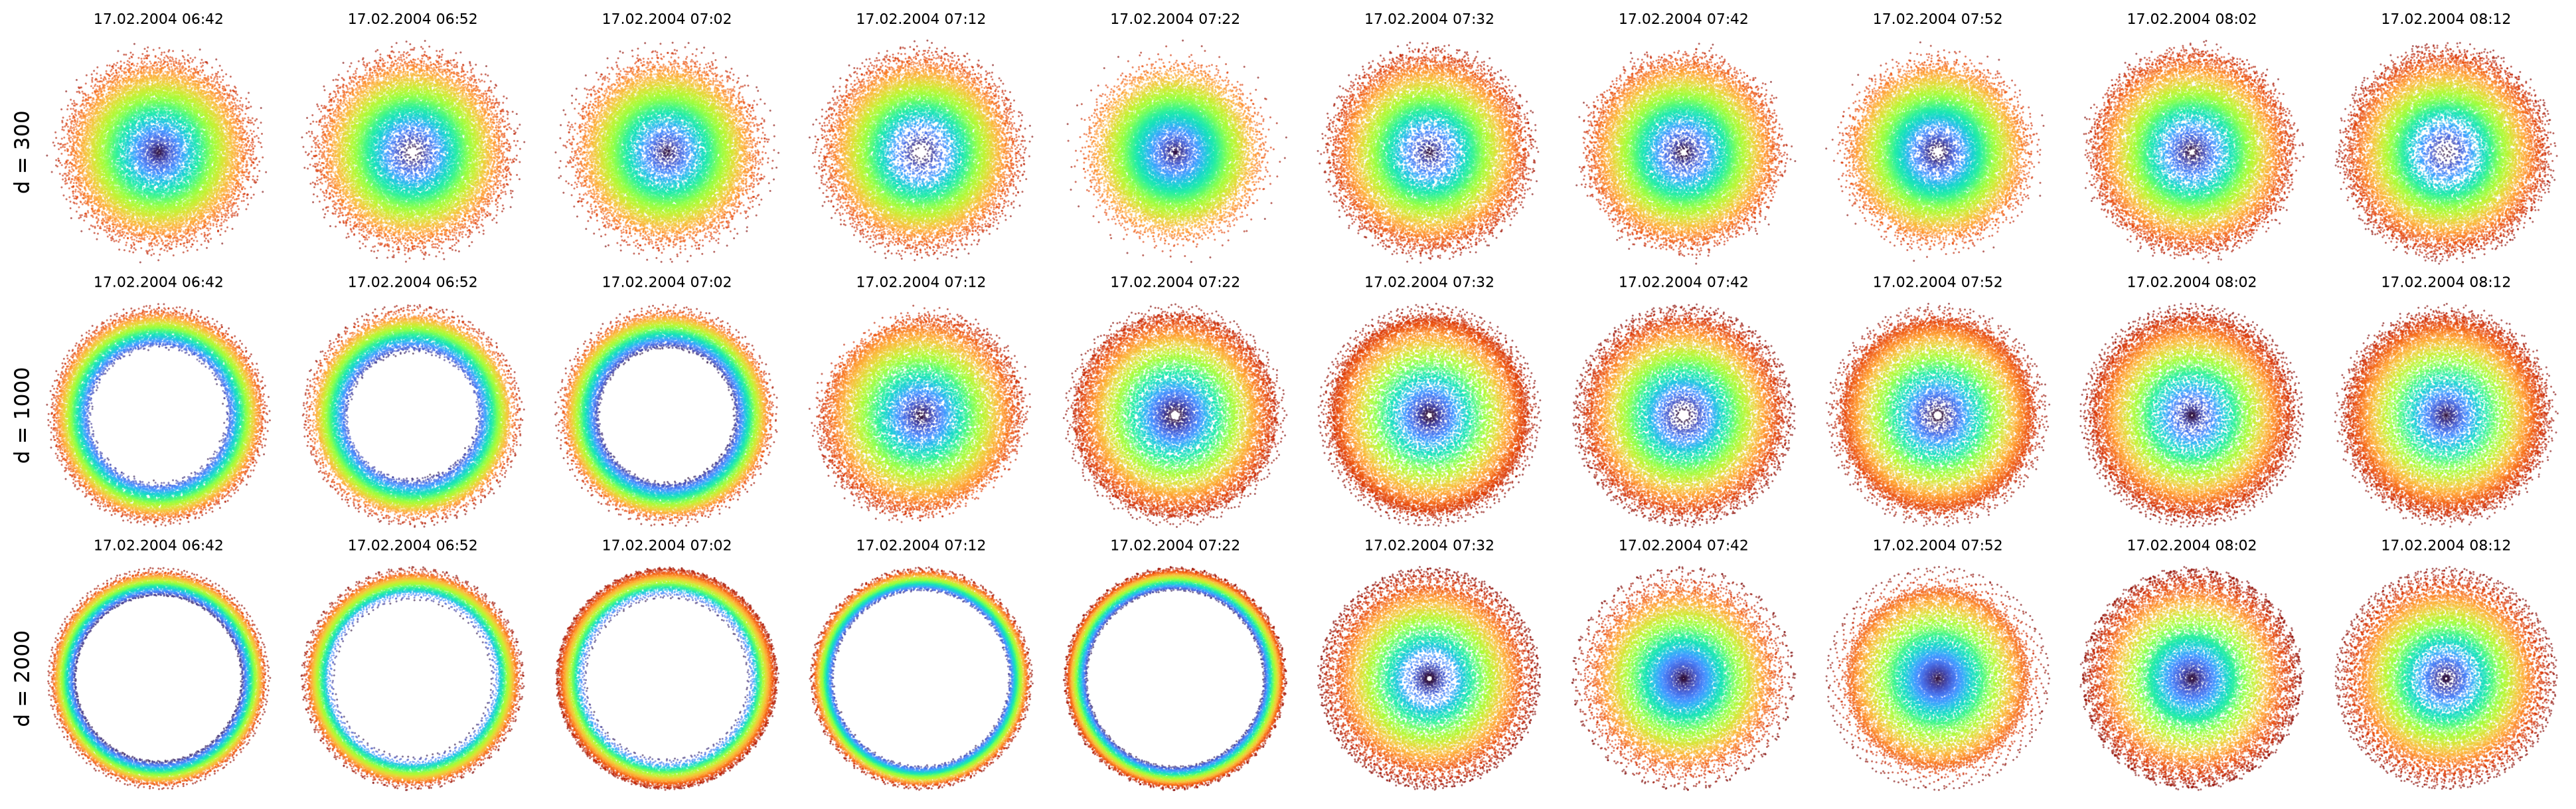
\includegraphics[width=\linewidth]{figures/differentParametersResults/dimensio_compare.png}
    \end{adjustwidth}
    \caption{Influence of the parameter w on the plots.}
    \label{fig:differentW}
\end{figure}
